\chapter{Hardware experiments}

The experiments were aimed at validation of the functionality of the designed and manufactured system. According to the plan, the system was first calibrated and tuned. Sensor calibration was conducted on a flat surface before mounting. Next, the fusion parameters were tuned when the sensor mounted on a robot traversed previously prepared trajectories.\\

First, the orientation estimation was examined. The node was rigidly linked to the robot gripper. Figure \ref{sensor_mount} presents the sensor mounted to the robot. The sponges were used to mitigate vibrations. Then, the robot executed a predetermined motion in which the position remained constant while only the orientation changed among five learned configurations. The orientation calculated by the robot control system was compared with the orientation estimated by the inertial sensors. Due to the lack of a magnetometer, the yaw angle could not be properly estimated, so its analyses were skipped. However, the yaw angle can be fixed by using an appropriate constraint (equation (\ref{yaw_constraint_fun})). The experiment was repeated without and with constraints correction and with various speeds. Listing \ref{karel1} presents the KAREL program that realizes this trajectory.
 
 \begin{figure}[!h]
 	\centering
 	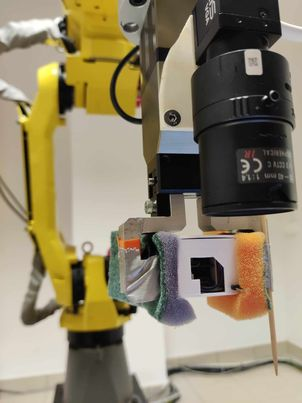
\includegraphics[width=0.42\textwidth]{sensor_mount.jpg}
 	\caption{Sensor mounted in the robot's gripper}
 	\label{sensor_mount}
 \end{figure}
 
 \begin{lstlisting}[caption={The KAREL program realizing an orientation changes}, captionpos=t, label=karel1]
	 1:  RUN PY_LOGGER;
	 2:  WAIT  15.00(sec);
	 3:  R[133]=50;
	 4:  J PR[54] 100% FINE;
	 5:  LBL[1:S];
	 6:  IF R[133]>100,JMP LBL[2];
	 7:  L PR[53] R[133]mm/sec FINE;
	 8:  L PR[54] R[133]mm/sec FINE;
	 9:  L PR[52] R[133]mm/sec FINE;
	10:  L PR[54] R[133]mm/sec FINE;
	11:  L PR[51] R[133]mm/sec FINE;
	12:  L PR[54] R[133]mm/sec FINE;
	13:  L PR[50] R[133]mm/sec FINE;
	14:  L PR[54] R[133]mm/sec FINE;
	15:  R[133]=R[133]+10;
	16:  JMP LBL[1];
	17:  LBL[2:E];
 \end{lstlisting}

Next, the system was examined under the default operating conditions to estimate the position and the orientation. The node was mounted on a plate that realizes a circular motion with different frequencies and directions, in accordance with the mechanism constraints. The estimation was conducted in multiple variants, which included:
\begin{itemize}
	\item case A -- position provider + gyroscope (the accelerometer was used only to correct orientation),
	\item case B -- position provider + gyroscope + accelerometer + constraint correction,
	\item case C -- position provider + constraint correction,
	\item case D -- position provider + gyroscope + accelerometer,
	\item case E -- position provider + gyroscope + accelerometer + constraint correction
	\item case F -- position provider + gyroscope + accelerometer + simplified constraint correction
\end{itemize}

The configuration without a position provider was also examined, but the results obtained were much worse in terms of quality. During the experiments, it was assumed that orientation does not change, and the position provider sample rate was limited to 2 Hz. The trajectory generated by the industrial robot is similar to that given in the equations (\ref{tcp_begin} - \ref{tcp_end}), but due to the robot control system limitations, the speed is discreetly increased twice per revolution. Listing \ref{karel2} presents the KAREL program that realizes this trajectory.

\begin{lstlisting}[caption={The KAREL program realizing a circular motion}, captionpos=t, label=karel2]
 	 1:  RUN PY_LOGGER;
	 2:  WAIT  15.00(sec);
	 3:  R[133]=30;
 	 4:  J PR[55] 100% FINE;
	 5:  LBL[1:S];
	 6:  IF R[133]>300,JMP LBL[2];
 	 7:  C PR[56]    
	  :  PR[57] R[133]mm/sec CNT100;
	 8:  R[133]=R[133]+10;
	 9:  C PR[58]    
	  :  PR[55] R[133]mm/sec CNT100;
	10:  R[133]=R[133]+10;
	11:  JMP LBL[1];
	12:  LBL[2:E];
\end{lstlisting}

\section{Results}

The gathered logs were post-processed and compared using MATLAB scripts. Figures \ref{ori_est_roll} - \ref{ori_est_yaw} present the orientation estimation from the first experiment. The estimated orientation angles are compared with the orientation calculated by the robot positioning system. However, as the notation used to describe orientation differ -- the system use quaternions, while the FANUC robot use W-P-R notation -- both orientations where transformed to more readable Euler angles (roll-pitch-yaw).  \\

Figures \ref{pos_est_x} - \ref{ori_est_yaw2} present the position and orientation estimations obtained for the proposed configuration. It is expected that x and y coordinates estimate circular motion while the z and orientation angles remain zeros.\\

The profit from the application of constraint correction is eminently visible when corrections with various "strengths" are compared. Figure \ref{corr_strength} presents an estimation of position in circular motion for different parameters (see equation \ref{constraint_final})). The sample rate of the external position provider is constant, so there are increasingly fewer updates for every rotation. If correction is inactive, the estimation tends to drift in the peaks. However, the "stronger" correction is active, the less error in these moments.

\begin{figure}[p]
	\centering
	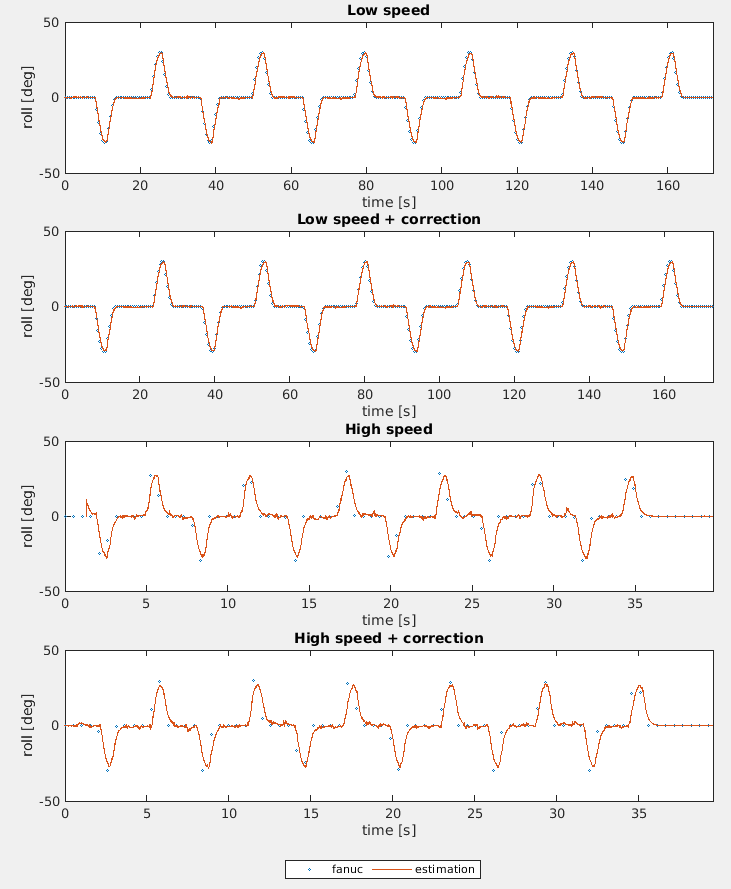
\includegraphics[width=\textwidth]{ori_est_roll.png}
	\caption{Experiment 1: orientation estimation -- roll}
	\label{ori_est_roll}
\end{figure}

\begin{figure}[p]
	\centering
	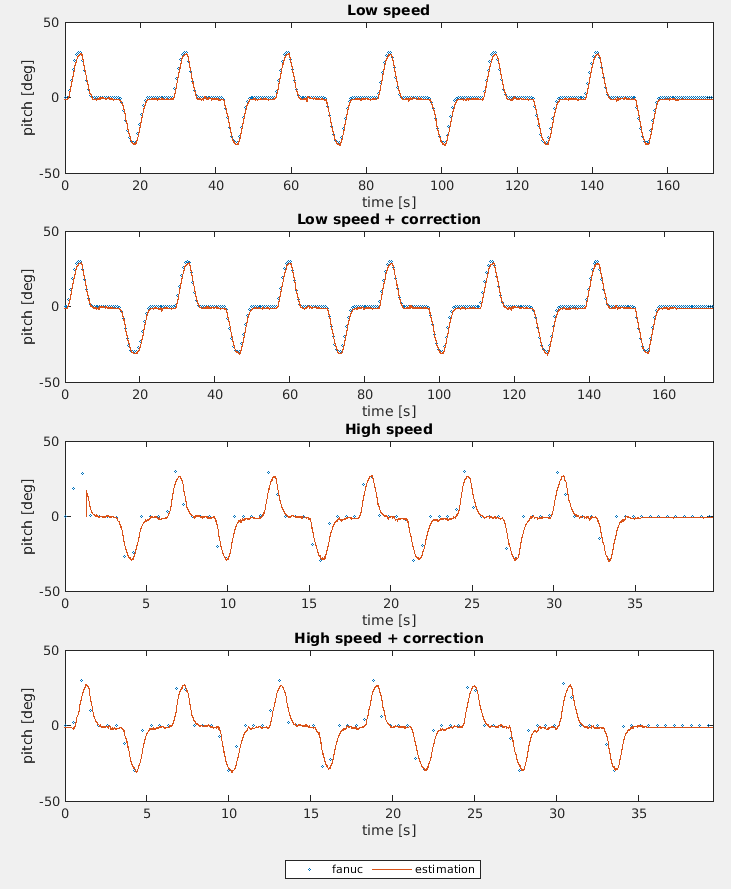
\includegraphics[width=\textwidth]{ori_est_pitch.png}
	\caption{Experiment 1: orientation estimation -- pitch}
	\label{ori_est_pitch}
\end{figure}


\begin{figure}[p]
	\centering
	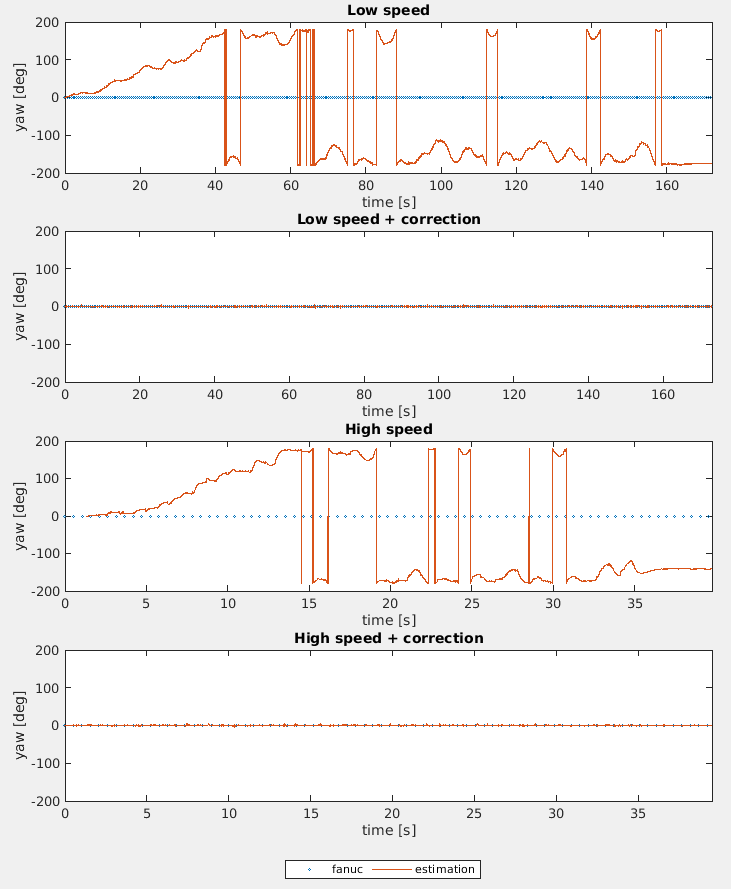
\includegraphics[width=\textwidth]{ori_est_yaw.png}
	\caption{Experiment 1: orientation estimation -- yaw}
	\label{ori_est_yaw}
\end{figure}

\begin{figure}[p]
	\centering
	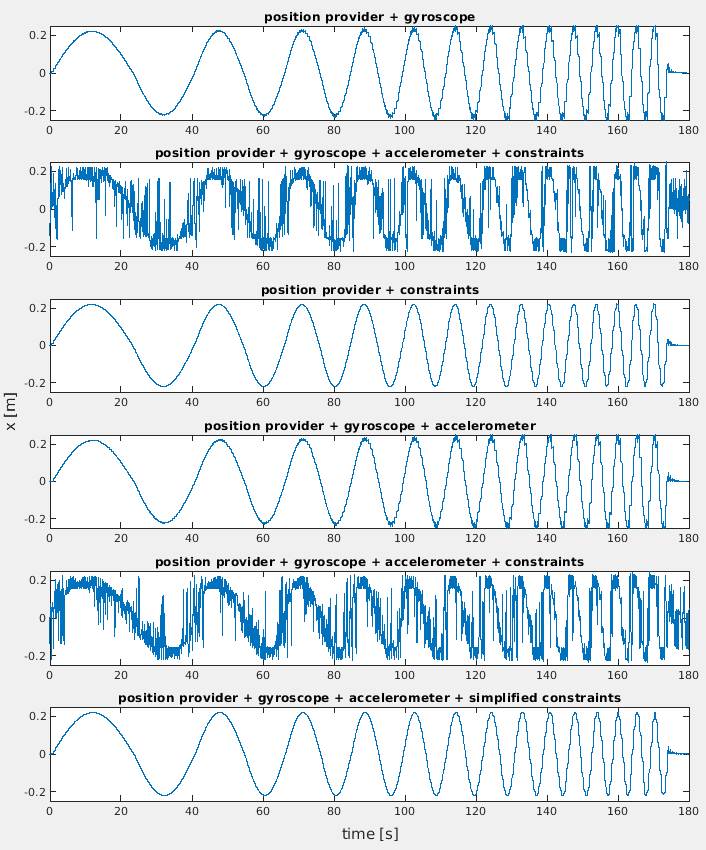
\includegraphics[width=\textwidth]{pos_est_x.png}
	\caption{Experiment 2: position estimation -- x}
	\label{pos_est_x}
\end{figure}

\begin{figure}[p]
	\centering
	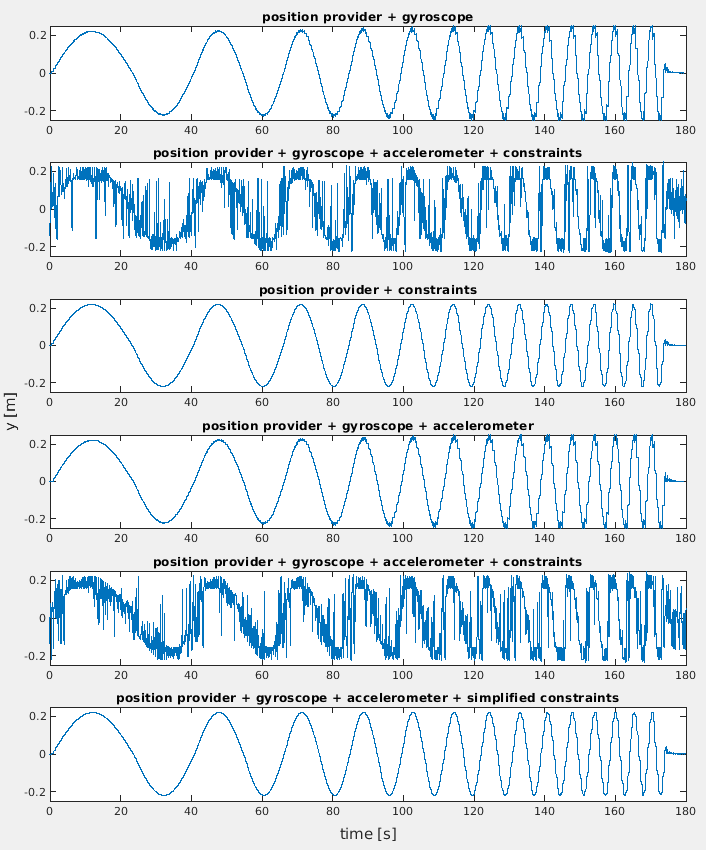
\includegraphics[width=\textwidth]{pos_est_y.png}
	\caption{Experiment 2: position estimation -- y}
	\label{pos_est_y}
\end{figure}

\begin{figure}[p]
	\centering
	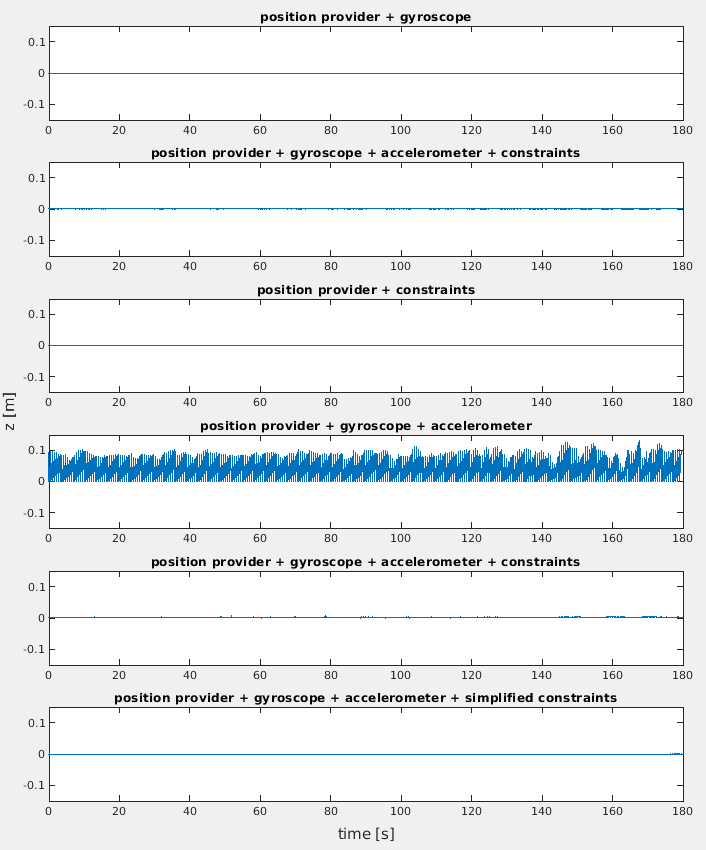
\includegraphics[width=\textwidth]{pos_est_z.png}
	\caption{Experiment 2: position estimation -- z}
	\label{pos_est_z}
\end{figure}

\begin{figure}[p]
	\centering
	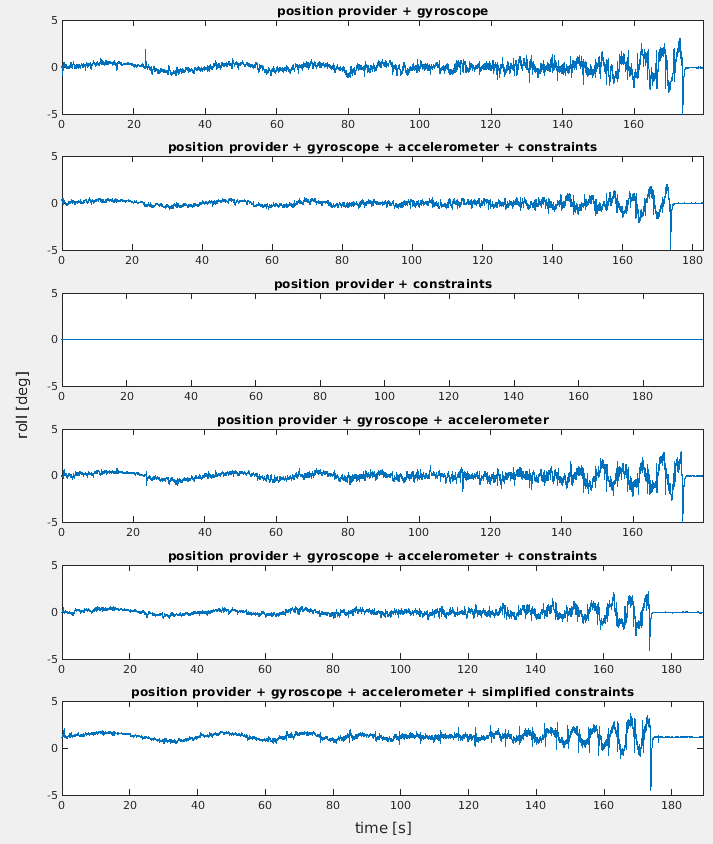
\includegraphics[width=\textwidth]{ori_est_roll2.png}
	\caption{Experiment 2: orientation estimation -- roll}
	\label{ori_est_roll2}
\end{figure}

\begin{figure}[p]
	\centering
	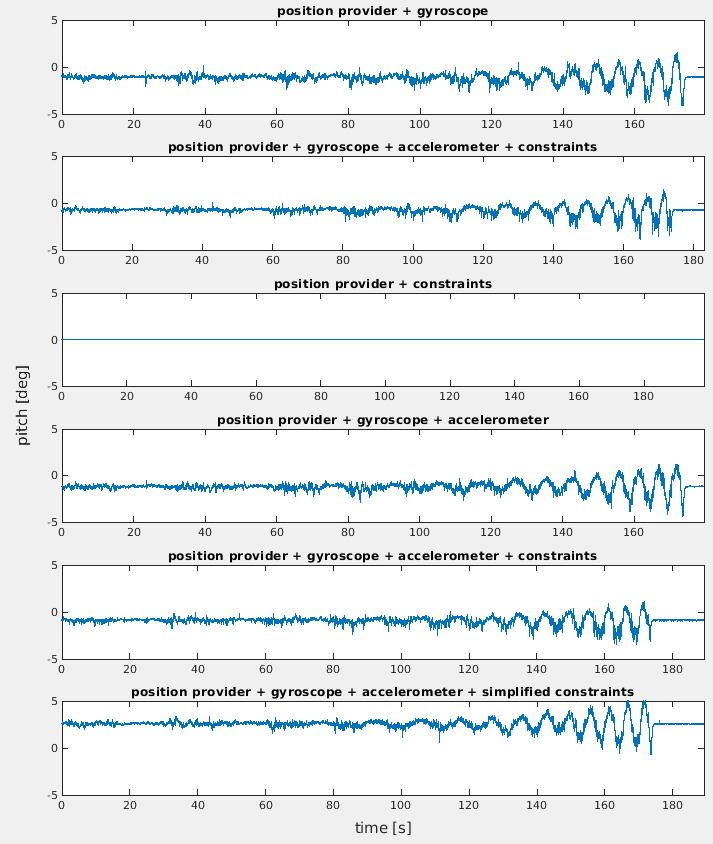
\includegraphics[width=\textwidth]{ori_est_pitch2.png}
	\caption{Experiment 2: orientation estimation -- pitch}
	\label{ori_est_pitch2}
\end{figure}


\begin{figure}[p]
	\centering
	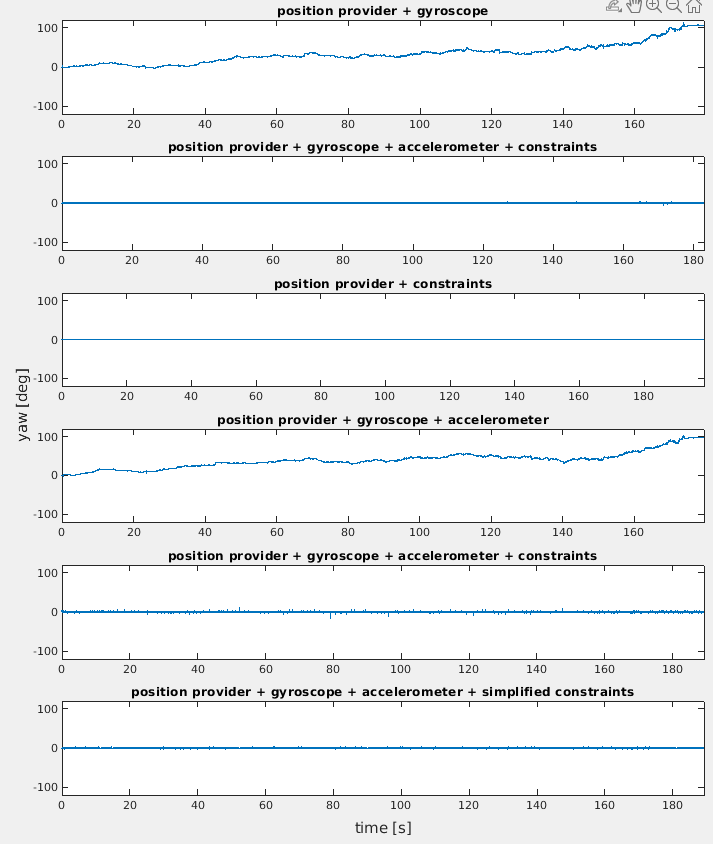
\includegraphics[width=\textwidth]{ori_est_yaw2.png}
	\caption{Experiment 2: orientation estimation -- yaw}
	\label{ori_est_yaw2}
\end{figure}


\begin{figure}[p]
	\centering
	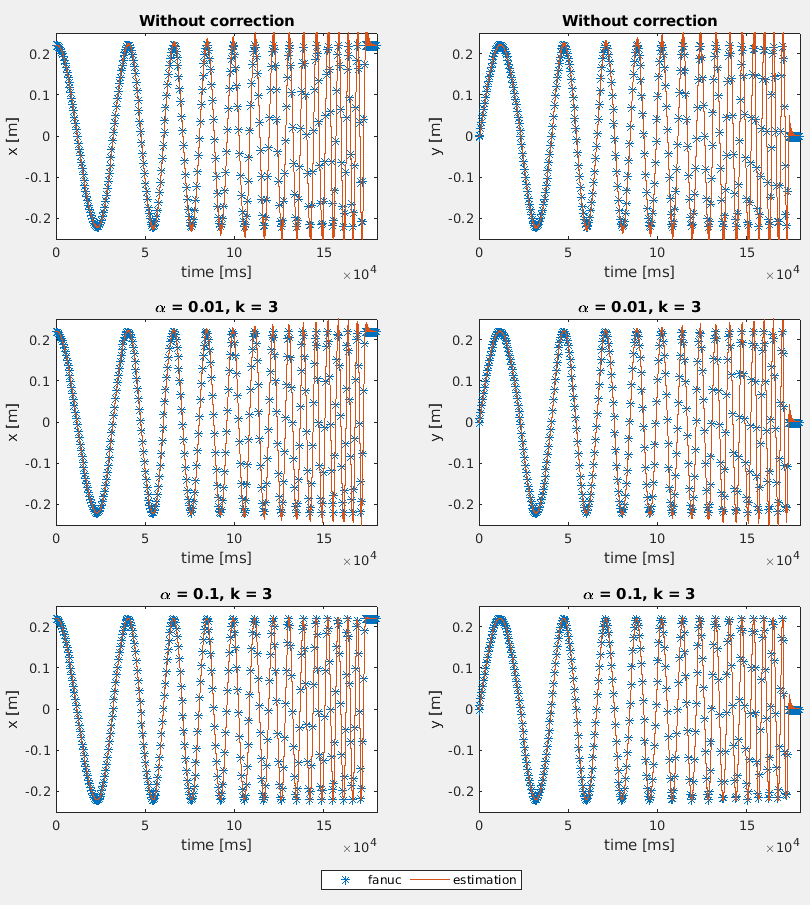
\includegraphics[width=\textwidth]{corr_influence.png}
	\caption{Tuning: the influence of constraints correction}
	\label{corr_strength}
\end{figure}

\section{Results discussion}

The first experiment showed that the system is able to provide adequate results based only on inertial sensors' readings. The estimation is reliable for slow and fast motions, where the fast motion is defined as a limit of the used industrial robot. However, in a minimal configuration, only roll and pitch angles can be estimated. In order to achieve full orientation estimation, additional system information is needed.\\

The second experiment reflected the behavior of the system under normal operating conditions. It turned out that in cases B and E, the estimated position was noise. The reason for that phenomenon is related to the properties of the system structure represented by constraints. For the examined mechanism, any orientation other than $\begin{bmatrix}0 & 0 & 0 \end{bmatrix}^T$ is strictly linked with a specified point in space (mind the alternative assembly of the system, corresponding to the alternative branch of bifurcation). Moreover, the implemented correction is more likely to change position than the orientation. As a result, when the orientation drifts, the correction tries to find the position that fulfills the constraint equations. To prove that hypothesis, case F was added to an experiment. It shows that if the orientation and position are not linked by constraints, the presence of the inertial sensor and the drifts do not lead to noisy estimation. The results cast doubt on the profitability of using an accelerometer in the prediction phase. Its presence leads to a disturbance in the z coordinate. However, this does not exclude accelerometer usage when correcting orientation. Furthermore, the influence of constraints correction is especially visible in the estimation amplitude.
  
Despite the described issues, it is possible to choose a variant without major defects.
The research conducted allows to conclude that the developed system can correctly estimate the position and orientation. 



